% !TeX program = lualatex
%******************************************************** -*-LaTeX-*- ******************************
%                                                                                                  *
% v1.1.2.6.9.1 Zehn.tex                                                                            *
%                                                                                                  *
% Copyright (C) 2024 Kategory GmbH \& Co. KG (joerg.kunze@kategory.de)                             *
%                                                                                                  *
% v1.1.2.6.9.1 Zehn is part of kategoryMathematik.                                                 *
%                                                                                                  *
% kategoryMathematik is free software: you can redistribute it and/or modify                       *
% it under the terms of the GNU General Public License as published by                             *
% the Free Software Foundation, either version 3 of the License, or                                *
% (at your option) any later version.                                                              *
%                                                                                                  *
% kategoryMathematik is distributed in the hope that it will be useful,                            *
% but WITHOUT ANY WARRANTY; without even the implied warranty of                                   *
% MERCHANTABILITY or FITNESS FOR A PARTICULAR PURPOSE.  See the                                    *
% GNU General Public License for more details.                                                     *
%                                                                                                  *
% You should have received a copy of the GNU General Public License                                *
% along with this program.  If not, see <http://www.gnu.org/licenses/>.                            *
%                                                                                                  *
%***************************************************************************************************

% !!!!!!!!!!!!!!!!!!!!!!!!!!!!!!!!!!!!!!!!!!!!!!!!!!!!!!!!!!!!!!!!!!!!!!!!!!!!!!!!!!!!!!!!!!!!!!!
% Wegen der hebräischen Schrift geht diese Datei nunr mit LuaLaTeX.
% deswegen die erste Zeile, damit TeXstudio den LuaLaTeX-Compiler nimmt
% Zusätzlich müssen wir den SBL Hebrew Font isntallieren.
% Den finden wir unter https://www.sbl-site.org/educational/biblicalfonts_sblhebrew.aspx
% Nach dem Download muss die Datei SBL_Hbrw.ttf in das Verzeichniss c:\Windows\Fonts kopiert werden
% Das ist aber auch im auf der selben Web-Seite zu findenen User Manual beschrieben.
% Wie es auf Linux oder Mac geht, können wir auch dort beschrieben finden. 
% Achte auch auf das \usepackage[utf8]{luainputenc}

\documentclass[a4paper]{amsart}
% \documentclass[a4paper]{book}

%-----------------------------------------------------------------------------------------------------*
% package:                                                                                            *
%-----------------------------------------------------------------------------------------------------*
\usepackage{amssymb}
\usepackage{amsfonts}
\usepackage{amsmath}
\usepackage{amsthm}

\usepackage{mathabx}

\usepackage{a4wide} % a little bit smaller margins

\usepackage{graphicx}
\usepackage{hyperref}
\usepackage{algorithmic}
\usepackage{listings}
\usepackage{color}
\usepackage{colortbl}
\usepackage{sidecap}
\usepackage{comment}
\usepackage{tcolorbox}
\usepackage{collect}

\usepackage{upgreek}

% \usepackage{diagrams}
\usepackage{luatextra}

\usepackage{polyglossia}
\usepackage[autostyle,german=guillemets]{csquotes}

\setmainlanguage[spelling=new]{german}
\setotherlanguage[variant=polytonic]{greek}

\newfontfamily\hebrewfont[Script=Hebrew,Scale=MatchUppercase,Ligatures=TeX]{SBL Hebrew}
\newcommand{\texthebrew}[1]{\bgroup\textdir TRT\hebrewfont #1\egroup}
\newenvironment{hebrew}{\textdir TRT\pardir TRT\hebrewfont}{}

\usepackage[none]{hyphenat}
\emergencystretch=4em

\usepackage[utf8]{luainputenc} % to be able to use äöü as characters in text
\usepackage[T1]{fontenc} % to be able to use äöü in lables
\usepackage{lmodern}     % to avoid pixelation introduced by fontenc

\usepackage{hyperref}

\usepackage{tikz}
\usepackage{tikz-cd}
\usetikzlibrary{shapes.geometric}

\usetikzlibrary{babel}

%-----------------------------------------------------------------------------------------------------*
% theorem:                                                                                            *
%-----------------------------------------------------------------------------------------------------*
\theoremstyle{definition}
\newtheorem{theorem}{Theorem}[subsection]

\newcommand{\myTheorem}[1]{%
  \newtheorem{jk#1}[theorem]{#1}
  \newenvironment{#1}[1]{%
    \expandafter\begin{jk#1} \expandafter\label{#1:##1}\textbf{(##1):}
  }{%
    \expandafter\end{jk#1}
  }
}

\myTheorem{Definition}
\myTheorem{Proposition}
\myTheorem{Theorem}
\myTheorem{Example}
\myTheorem{Remark}

\definecollection{jkjkFrage}
\newtheorem{jkFrage}[theorem]{Frage}
\newenvironment{Frage}[1]{%
  \expandafter\begin{jkFrage} \expandafter\label{Frage:#1}\textbf{(#1):}
  \begin{collect}{jkjkFrage}{}{}
    \item \ref{Frage:#1} #1
  \end{collect}
}{%
  \expandafter\end{jkFrage}
}

\newcommand{\myRef}[2]{[#1 \ref{#1:#2}, ``#2'']}

\renewcommand{\proofname}{Beweis}

%-----------------------------------------------------------------------------------------------------*
% operator:                                                                                           *
%-----------------------------------------------------------------------------------------------------*
\DeclareMathOperator{\End}{End}
\DeclareMathOperator{\Ker}{Ker}
\DeclareMathOperator{\Mat}{Mat}
\DeclareMathOperator{\rank}{rank}
\DeclareMathOperator{\ggT}{ggT}
\DeclareMathOperator{\len}{len}
\DeclareMathOperator{\ord}{ord}
\DeclareMathOperator{\kgV}{kgV}
\DeclareMathOperator{\id}{id}
\DeclareMathOperator{\red}{red}
\DeclareMathOperator{\supp}{supp}
\DeclareMathOperator{\Bild}{Bild}
\DeclareMathOperator{\Rang}{Rang}
\DeclareMathOperator{\Det}{Det}
\DeclareMathOperator{\Hom}{Hom}

\DeclareMathOperator{\sub}{sub}
\DeclareMathOperator{\blk}{blk}
\DeclareMathOperator{\minimal}{minimal}
\DeclareMathOperator{\maximal}{maximal}

\definecolor{mygreen}{rgb}{0,0.6,0}
\definecolor{mygray}{rgb}{0.5,0.5,0.5}
\definecolor{mymauve}{rgb}{0.58,0,0.82}

\lstset{ %
  backgroundcolor=\color{white},   % choose the background color
  basicstyle=\ttfamily\footnotesize,        % size of fonts used for the code
  breaklines=true,                 % automatic line breaking only at whitespace
  captionpos=b,                    % sets the caption-position to bottom
  commentstyle=\color{mygreen},    % comment style
  escapeinside={\%*}{*)},          % if you want to add LaTeX within your code
  keywordstyle=\color{blue},       % keyword style
  stringstyle=\color{mymauve},     % string literal style
  frame=single
}

\setcounter{MaxMatrixCols}{20}

%******************************************************************************************************
%                                                                                                     *
% definition:                                                                                         *
%                                                                                                     *
%******************************************************************************************************
\newcommand{\R}{\ensuremath{\mathbb{ R }}}
\newcommand{\Q}{\ensuremath{\mathbb{ Q }}}
\newcommand{\Z}{\ensuremath{\mathbb{ Z }}}
\newcommand{\N}{\ensuremath{\mathbb{ N }}}
\newcommand{\C}{\ensuremath{\mathbb{ C }}}
\newcommand{\A}{\ensuremath{\mathbb{ A }}}
\newcommand{\F}{\ensuremath{\mathbb{ F }}}
\newcommand{\K}{\ensuremath{\mathbb{ K }}}
\newcommand{\Pb}{\ensuremath{\mathbb{ P }}}

\newcommand{\M}{\ensuremath{\mathcal{ M }}}
\newcommand{\V}{\ensuremath{\mathcal{ V }}}

\newcommand{\AAA}{\ensuremath{\mathcal{ A }}}
\newcommand{\BB}{\ensuremath{\mathcal{ B }}}
\newcommand{\CC}{\ensuremath{\mathcal{ C }}}
\newcommand{\EE}{\ensuremath{\mathcal{ E }}}
\newcommand{\KK}{\ensuremath{\mathcal{ K }}}
\newcommand{\MM}{\ensuremath{\mathcal{ M }}}
\newcommand{\PP}{\ensuremath{\mathcal{ P }}}
\newcommand{\ZZ}{\ensuremath{\mathcal{ Z }}}

\newcommand{\imporant}[1]{ \textcolor{red}{\textbf{#1}} }

\newcommand{\bb}[1]{\mathbf{#1}}
\newcommand{\balpha}{\boldsymbol{\upalpha}}
\newcommand{\bbeta}{\boldsymbol{\upbeta}}
\newcommand{\bgamma}{\boldsymbol{\upgamma}}
\newcommand{\bdelta}{\boldsymbol{\delta}}
\newcommand{\bmu}{\boldsymbol{\upmu}}

\newcommand{\z}[1]{\Z_{#1}}
\newcommand{\e}[1]{\z{#1}^*}
\newcommand{\q}[1]{(\e{#1})^2}

\excludecomment{book}
\excludecomment{example}
\excludecomment{backup}

\begin{document}

%******************************************************************************************************
%                                                                                                     *
\begin{titlepage}
%                                                                                                     *
%******************************************************************************************************
% \vspace*{\fill}
\centering
{\huge
(Grund) Zahlen\\[1cm]
\textbf{v1.1.2.6.9.1 Zehn}
}\\[1cm]

\textbf{Kategory GmbH \& Co. KG}\\
Präsentiert von Jörg Kunze\\
Copyright (C) 2024 Kategory GmbH \& Co. KG

\end{titlepage}

%\clearpage
%\setcounter{page}{2}
%
%\tableofcontents

\newpage

%******************************************************************************************************
%                                                                                                     *
\section*{Beschreibung}
%                                                                                                     *
%******************************************************************************************************

%******************************************************************************************************
\subsection*{Inhalt}
%******************************************************************************************************
Die ||||| ||||| (10, Zehn) ist der Nachfolger von ||||| |||| (9, Neun). Die Zehn ist die erste Zahl, die keine Ziffer ist. Wir benötigen zwei Ziffern, um sie zu schreiben.

Die meisten Menschen haben zehn Finger und zehn Zehen. Die Zehn ist Namensgeber und Basis unseres Zehnersystems. 

Die Zehn ist die elfte Zahl. Es gibt 11 (elf) Befüllungszustände, wenn wir 10 (zehn) Plätze befüllen können.

%******************************************************************************************************
\subsection*{Präsentiert}
%******************************************************************************************************
Von Jörg Kunze

%******************************************************************************************************
\subsection*{Voraussetzungen}
%******************************************************************************************************
Schulmathematik, Zählen, ein wenig rechnen mit Strichen und Punkten, Zählen, Addieren, Pack-Schreibweise von Zahlen.

%******************************************************************************************************
\subsection*{Text}
%******************************************************************************************************
Der Begleittext als PDF und als LaTeX findet sich unter
\url{https://github.com/kategory/kategoryMathematik/tree/main/v1%20Grund/v1.1%20Zahlen/v1.1.2.6.9%20Neun}.

%******************************************************************************************************
\subsection*{Meine Videos}
%******************************************************************************************************
Siehe auch in den folgenden Videos:\\
v1.1.2.5.6.1 (Grund) Zahlen - Darstellung\\
\url{https://youtu.be/t8cyZevFWFs}\\
\\
v1.1.2.5.6 (Grund) Zahlen - Pack Schreibweise\\
\url{https://youtu.be/OGXoLiBL2MQ}\\
\\
v1.1.2.4 (Grund) Zählen\\
\url{ttps://youtu.be/I6iIG2ZtPCU}\\

%******************************************************************************************************
\subsection*{Quellen}
%******************************************************************************************************
Siehe auch in den folgenden Seiten:\\
\url{https://de.wikipedia.org/wiki/Neun}\\
\url{https://de.wikipedia.org/wiki/Muse_(Mythologie)}\\
\url{https://de.wikipedia.org/wiki/Ramadan}\\

%******************************************************************************************************
\subsection*{Buch}
%******************************************************************************************************
Grundlage ist folgendes Buch:\\
"`Basiswissen Grundschule – Mathematik"'\\
Ute Müller-Wolfangel, Beate Schreiber\\
2014\\
Bibliographisches Institut\\
978-3-411-72063-7 (ISBN)
\\
\url{https://www.lehmanns.de/shop/schulbuch-lexikon-woerterbuch/28535581-9783411720637-basiswissen-grundschule-mathematik}

%******************************************************************************************************
\subsection*{Lizenz}
%******************************************************************************************************
Dieser Text und das Video sind freie Software. Sie können es unter den Bedingungen der 
GNU General Public License, wie von der Free Software Foundation veröffentlicht, weitergeben 
und/oder modifizieren, entweder gemäß Version 3 der Lizenz oder (nach Ihrer Option) jeder späteren Version.

Die Veröffentlichung von Text und Video erfolgt in der Hoffnung, dass es Ihnen von Nutzen sein wird, 
aber OHNE IRGENDEINE GARANTIE, sogar ohne die implizite Garantie der MARKTREIFE oder der 
VERWENDBARKEIT FÜR EINEN BESTIMMTEN ZWECK. Details finden Sie in der GNU General Public License.

Sie sollten ein Exemplar der GNU General Public License zusammen mit diesem Text erhalten haben 
(zu finden im selben Git-Projekt). 
Falls nicht, siehe \url{http://www.gnu.org/licenses/}.

Bild "`Hände"' gefunden auf \url{https://he.wikipedia.org/wiki/%D7%9B%D7%A3_%D7%A8%D7%92%D7%9C}.

Bild "`Füße"' von \url{https://unsplash.com/de/\@jibarox?utm_content=creditCopyText\&utm_medium=referral\&utm_source=unsplash} Luis Quintero auf \url{https://unsplash.com/de/fotos/menschenhand-qKspdY9XUzs?utm\_content=creditCopyText\&utm_medium=referral\&utm\_source=unsplash} Unsplash

%******************************************************************************************************
\subsection*{Das Video}
%******************************************************************************************************
Das Video hierzu ist zu finden unter \url{https://youtu.be/V0_h8WZrkos}

%******************************************************************************************************
%                                                                                                     *
\section{Neun}
%                                                                                                     *
%******************************************************************************************************
\def\kategoryVspace{5pt}

%******************************************************************************************************
\subsection{Striche}
%******************************************************************************************************
\begin{tikzpicture}
\draw (0.0, 0) -- (0.0, 0.4);
\draw (0.1, 0) -- (0.1, 0.4);
\draw (0.2, 0) -- (0.2, 0.4);
\draw (0.3, 0) -- (0.3, 0.4);
\draw (0.4, 0) -- (0.4, 0.4);
\draw (0.5, 0) -- (0.5, 0.4);
\draw (0.6, 0) -- (0.6, 0.4);
\draw (0.7, 0) -- (0.7, 0.4);
\draw (0.8, 0) -- (0.8, 0.4);
\end{tikzpicture}
=
\begin{tikzpicture}
   \draw (0.0, 0) -- (0.0, 0.4);
   \draw (0.1, 0) -- (0.1, 0.4);
   \draw (0.2, 0) -- (0.2, 0.4);
   \draw (0.3, 0) -- (0.3, 0.4);
   \draw (0.4, 0) -- (0.4, 0.4);
   \draw (0.7, 0) -- (0.7, 0.4);
   \draw (0.8, 0) -- (0.8, 0.4);
   \draw (0.9, 0) -- (0.9, 0.4);
   \draw (1.0, 0) -- (1.0, 0.4);
\end{tikzpicture}
=
\begin{tikzpicture}
   \draw (0.05, 0) -- (0.05, 0.4);
   \draw (0.15, 0) -- (0.15, 0.4);
   \draw (0.25, 0) -- (0.25, 0.4);
   \draw (0.35, 0) -- (0.35, 0.4);
   \draw (0.40, 0) -- (0.00, 0.4);
   \draw (0.60, 0) -- (0.60, 0.4);
   \draw (0.70, 0) -- (0.70, 0.4);
   \draw (0.80, 0) -- (0.80, 0.4);
   \draw (0.90, 0) -- (0.90, 0.4);
\end{tikzpicture}

%******************************************************************************************************
\subsection{Kreisbild}
%******************************************************************************************************
\begin{tikzpicture}
   \draw [blue, fill=blue] (0.0, 2) circle (0.3);
   \draw [blue, fill=blue] (0.7, 2) circle (0.3);
   \draw [blue, fill=blue] (1.4, 2) circle (0.3);
   \draw [blue, fill=blue] (2.1, 2) circle (0.3);
   \draw [blue, fill=blue] (2.8, 2) circle (0.3);
   \draw [red , fill=red ] (3.5, 2) circle (0.3);
   \draw [red , fill=red ] (4.2, 2) circle (0.3);
   \draw [red , fill=red ] (4.9, 2) circle (0.3);
   \draw [red , fill=red ] (5.6, 2) circle (0.3);
   \draw [red            ] (6.3, 2) circle (0.3);
\end{tikzpicture}

Das Kreisbild und das Schreiben in Fünfer-Blöcken dient der Vorbereitung auf das Rechnen im Zehnersystem. Es zeigt Eigenschaften, die nicht zum inneren Wesen der Zahl gehören, sondern zu ihrem Verhältnis zum Zehnersystem. 

%******************************************************************************************************
\subsubsection{Kreisbild als Rechnung}
%******************************************************************************************************
\begin{tikzpicture}
   \draw (0.05, 0) -- (0.05, 0.4);
   \draw (0.15, 0) -- (0.15, 0.4);
   \draw (0.25, 0) -- (0.25, 0.4);
   \draw (0.35, 0) -- (0.35, 0.4);
   \draw (0.40, 0) -- (0.00, 0.4);

   \draw (0.60, 0) -- (0.60, 0.4);
   \draw (0.70, 0) -- (0.70, 0.4);
   \draw (0.80, 0) -- (0.80, 0.4);
   \draw (0.90, 0) -- (0.90, 0.4);
\end{tikzpicture}
=
\begin{tikzpicture}
   \draw (0.05, 0) -- (0.05, 0.4);
   \draw (0.15, 0) -- (0.15, 0.4);
   \draw (0.25, 0) -- (0.25, 0.4);
   \draw (0.35, 0) -- (0.35, 0.4);
   \draw (0.40, 0) -- (0.00, 0.4);
\end{tikzpicture}
+
\begin{tikzpicture}
   \draw (0.0, 0) -- (0.0, 0.4);
   \draw (0.1, 0) -- (0.1, 0.4);
   \draw (0.2, 0) -- (0.2, 0.4);
   \draw (0.3, 0) -- (0.3, 0.4);
\end{tikzpicture}
,
\begin{tikzpicture}
   \draw (0.05, 0) -- (0.05, 0.4);
   \draw (0.15, 0) -- (0.15, 0.4);
   \draw (0.25, 0) -- (0.25, 0.4);
   \draw (0.35, 0) -- (0.35, 0.4);
   \draw (0.40, 0) -- (0.00, 0.4);
   
   \draw (0.60, 0) -- (0.60, 0.4);
   \draw (0.70, 0) -- (0.70, 0.4);
   \draw (0.80, 0) -- (0.80, 0.4);
   \draw (0.90, 0) -- (0.90, 0.4);
\end{tikzpicture}
+
\begin{tikzpicture}
   \draw (0.0, 0) -- (0.0, 0.4);
\end{tikzpicture}
=
\begin{tikzpicture}
   \draw (0.05, 0) -- (0.05, 0.4);
   \draw (0.15, 0) -- (0.15, 0.4);
   \draw (0.25, 0) -- (0.25, 0.4);
   \draw (0.35, 0) -- (0.35, 0.4);
   \draw (0.40, 0) -- (0.00, 0.4);
   
   \draw (0.65, 0) -- (0.65, 0.4);
   \draw (0.75, 0) -- (0.75, 0.4);
   \draw (0.85, 0) -- (0.85, 0.4);
   \draw (0.95, 0) -- (0.95, 0.4);
   \draw (0.60, 0) -- (1.00, 0.4);
\end{tikzpicture}

Hier sehen wir nochmal schön, wie einfach die Rechnung $9 = 5+4$ ist, wenn wir die Zahlen als das sehen, was sie wirklich sind.

%******************************************************************************************************
\subsection{Zweiteilungen}
%******************************************************************************************************
\begin{tikzpicture}
   \draw (0.05, 0) -- (0.05, 0.4);
\end{tikzpicture}
+
\begin{tikzpicture}
   \draw (0.05, 0) -- (0.05, 0.4);
   \draw (0.15, 0) -- (0.15, 0.4);
   \draw (0.25, 0) -- (0.25, 0.4);
   \draw (0.35, 0) -- (0.35, 0.4);
   \draw (0.40, 0) -- (0.00, 0.4);
   
   \draw (0.60, 0) -- (0.60, 0.4);
   \draw (0.70, 0) -- (0.70, 0.4);
   \draw (0.80, 0) -- (0.80, 0.4);
\end{tikzpicture}
,
\begin{tikzpicture}
   \draw (0.05, 0) -- (0.05, 0.4);
   \draw (0.15, 0) -- (0.15, 0.4);
\end{tikzpicture}
+
\begin{tikzpicture}
   \draw (0.05, 0) -- (0.05, 0.4);
   \draw (0.15, 0) -- (0.15, 0.4);
   \draw (0.25, 0) -- (0.25, 0.4);
   \draw (0.35, 0) -- (0.35, 0.4);
   \draw (0.40, 0) -- (0.00, 0.4);
   
   \draw (0.60, 0) -- (0.60, 0.4);
   \draw (0.70, 0) -- (0.70, 0.4);
\end{tikzpicture}
,
\begin{tikzpicture}
   \draw (0.05, 0) -- (0.05, 0.4);
   \draw (0.15, 0) -- (0.15, 0.4);
   \draw (0.25, 0) -- (0.25, 0.4);
\end{tikzpicture}
+
\begin{tikzpicture}
   \draw (0.05, 0) -- (0.05, 0.4);
   \draw (0.15, 0) -- (0.15, 0.4);
   \draw (0.25, 0) -- (0.25, 0.4);
   \draw (0.35, 0) -- (0.35, 0.4);
   \draw (0.40, 0) -- (0.00, 0.4);
   
   \draw (0.60, 0) -- (0.60, 0.4);
\end{tikzpicture}
,
\begin{tikzpicture}
   \draw (0.05, 0) -- (0.05, 0.4);
   \draw (0.15, 0) -- (0.15, 0.4);
   \draw (0.25, 0) -- (0.25, 0.4);
   \draw (0.35, 0) -- (0.35, 0.4);
\end{tikzpicture}
+
\begin{tikzpicture}
   \draw (0.05, 0) -- (0.05, 0.4);
   \draw (0.15, 0) -- (0.15, 0.4);
   \draw (0.25, 0) -- (0.25, 0.4);
   \draw (0.35, 0) -- (0.35, 0.4);
   \draw (0.40, 0) -- (0.00, 0.4);
\end{tikzpicture}

%******************************************************************************************************
\subsection{Eck}
%******************************************************************************************************
Das regelmäßige 9-Eck:
\vspace{\kategoryVspace}

\begin{tikzpicture}
   \node[draw,minimum size=2cm,regular polygon,regular polygon sides=9, style={
      color = green,
      draw,
      line width = .05cm,
      inner xsep = 2.5cm,
      inner ysep = 0.5cm
   }] (a) {};
   
   \node[draw,minimum size=2cm,regular polygon,regular polygon sides=9, style={
      color = black,
      draw=none,
      line width = .01cm,
      inner xsep = 2.47cm,
      inner ysep = 0.5cm
   }] (b) {};

   \foreach \x in {1,2,...,9}
      \fill[orange] (b.corner \x) circle[radius=4pt];
   
\end{tikzpicture}

%******************************************************************************************************
\subsection{Ziffer}
%******************************************************************************************************
Die Zahl als Ziffer:
\vspace{\kategoryVspace}

{\Huge 9}

%******************************************************************************************************
\subsection{Rechnung mit Ziffern}
%******************************************************************************************************

%******************************************************************************************************
\subsubsection{Kreisbild als Rechnung mit Ziffern}
%******************************************************************************************************
$5 + 4 = 9$ und $9 + 1 = 10$
%******************************************************************************************************
\subsubsection{Zweiteilung als Rechnung mit Ziffern}
%******************************************************************************************************
$9 = 1 + 8 = 2 + 7 = 3 + 6 = 4 + 5$

%******************************************************************************************************
\subsection{Namen}
%******************************************************************************************************
Die Namen der Neun in verschiedenen Sprachen:
\vspace{\kategoryVspace}

\begin{tabular}{|c|c|c|}
   \hline
   \textbf{Sprache}& \textbf{Schreiben} & \textbf{Sprechen} \\
   \hline
   Deutsch     &Neun   &noin      \\
   \hline
   Englisch    &nine   &nain      \\
   \hline
   Französisch &neuf   &nöff      \\
   \hline
   Latein      &novem  &nowem     \\
   \hline
   Hebräisch   &\texthebrew{תשע}    &tescha' \\
   \hline
   Schwedisch  &nio    &nie'jä     \\
   \hline
\end{tabular}

%******************************************************************************************************
\subsection{Im Alltag}
%******************************************************************************************************
% 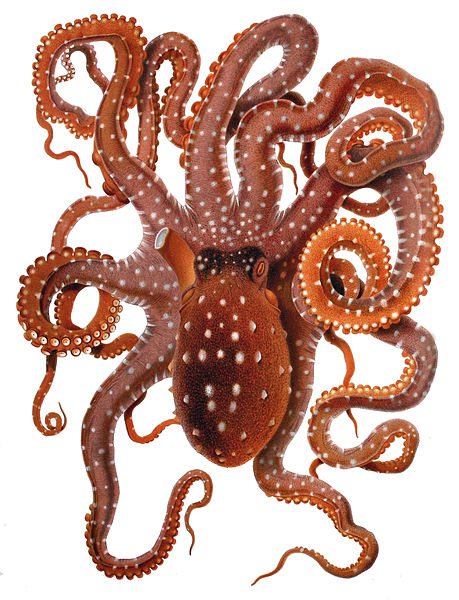
\includegraphics[height=4cm]{Octopus.jpg}


Der Ramadan (arabisch: heißer Monat) ist der Fastenmonat der Muslime und neunter 
Monat des islamischen Mondkalenders. In ihm wurde der Koran herabgesandt.

Die neun Musen:
\begin{enumerate}
   \item Klio, die Rühmende, ist die Muse der Geschichtsschreibung (Attribute: Papierrolle und Schreibgriffel);
   \item Euterpe, die Erfreuende, ist die Muse der Lyrik und des Flötenspiels (Attribut: Aulos, die Doppelflöte);
   \item Melpomene, die Singende, ist die Muse der Tragödie (Attribut: ernste Theatermaske, Weinlaubkranz, wahrscheinlich auch ein Schwert oder eine Keule);
   \item Erato, die Liebevolle, Sehnsucht Weckende, ist die Muse der Liebesdichtung (Attribut: Saiteninstrument, Leier);
   \item Terpsichore, die fröhlich im Reigen Tanzende, ist die Muse für Chorlyrik und Tanz (Attribut: Leier);
   \item Urania, die Himmlische, ist die Muse der Astronomie (Attribut: Himmelskugel und Zeigestab);
   \item Thalia, die Festliche, die Blühende, ist die Muse der Komödie (Attribut: lachende Theatermaske, Efeukranz und Krummstab, denn auch die heitere bukolische Poesie gehört zu ihr);
   \item Polyhymnia, die Hymnenreiche (Liederreiche). Sie ist die Muse des Gesangs mit der Leier (kein spezifisches Attribut, manchmal die Leier);
   \item Kalliope, die mit der schönen Stimme, ist die Muse der epischen Dichtung, der Rhetorik, der Philosophie und der Wissenschaft (Attribut: Schreibtafel und Schreibgriffel).
\end{enumerate}

\begin{figure}
   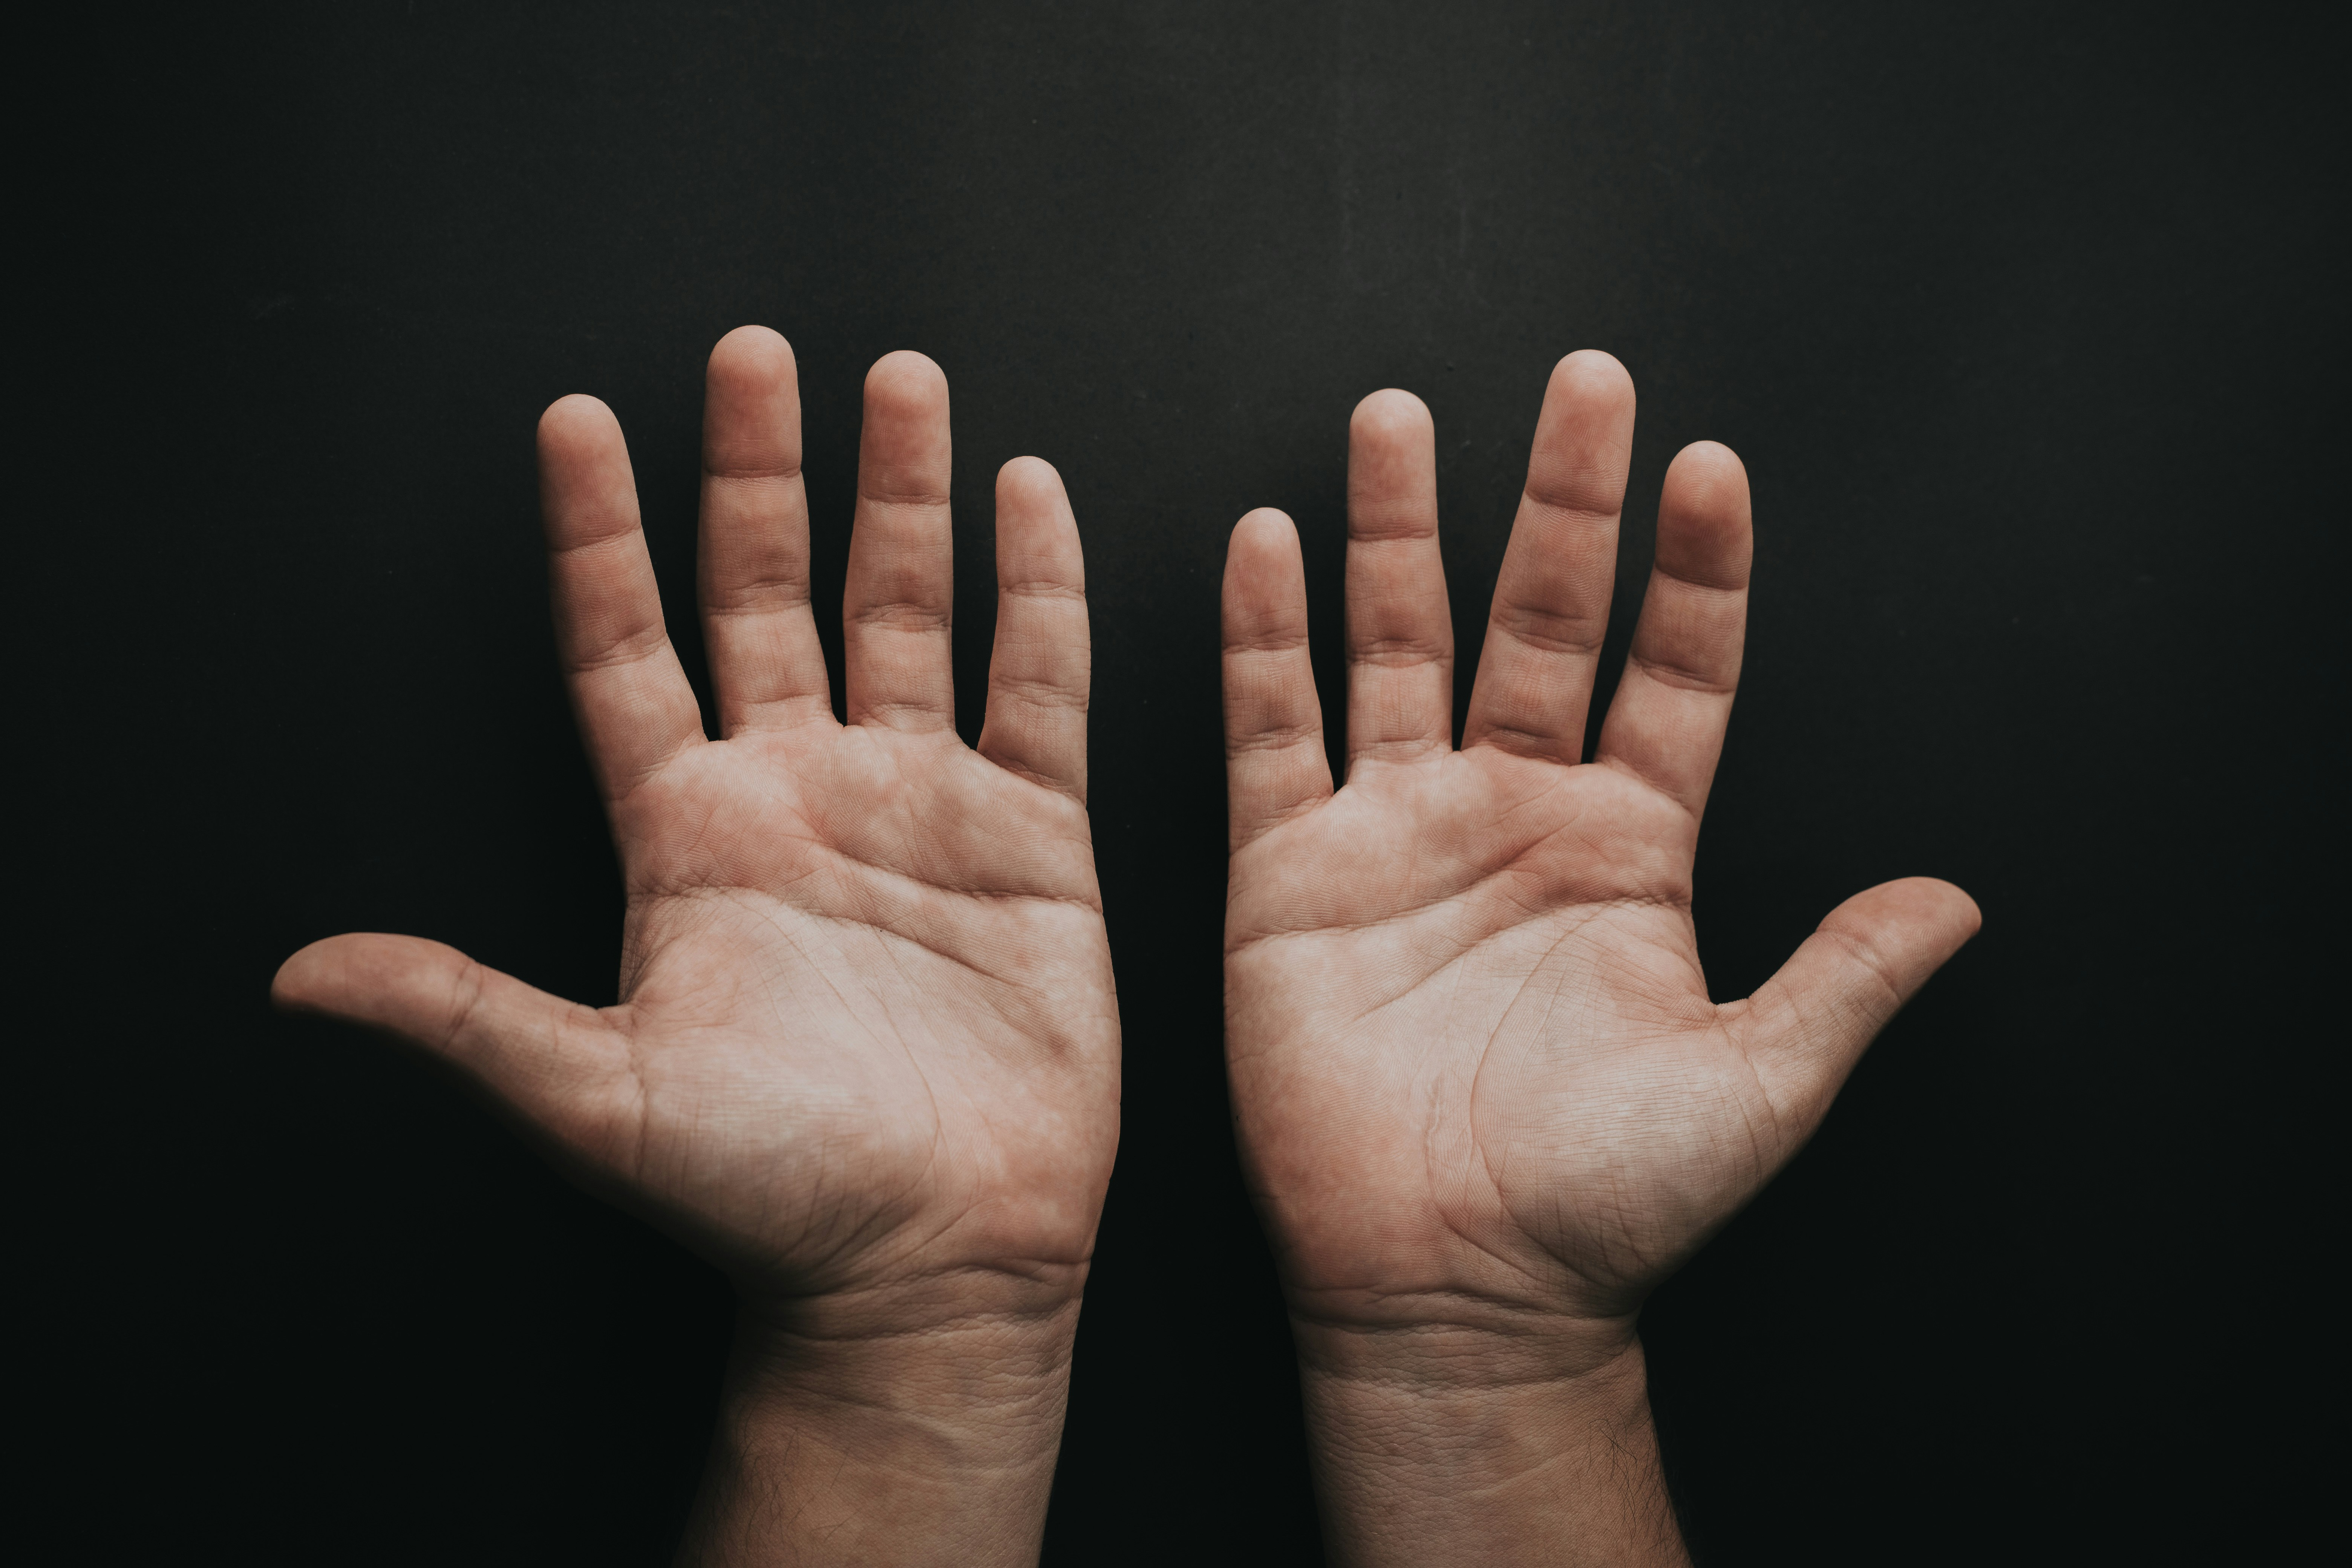
\includegraphics[height=6cm]{zehnFinger luis-quintero-qKspdY9XUzs-unsplash.jpg}
   \caption{Hände}
\end{figure}


\begin{figure}
   \includegraphics[height=6cm]{zehnZehen.jpg}
   \caption{Füße}
\end{figure}

%******************************************************************************************************
\subsection{In uns}
%******************************************************************************************************
nix.

%******************************************************************************************************
\subsection{Additionsverhalten}
%******************************************************************************************************
Keine Besonderheiten.

%******************************************************************************************************
\subsection{Multiplikationsverhalten}
%******************************************************************************************************
Keine Besonderheiten.

%******************************************************************************************************
\subsection{Das kleine Null-plus-Acht}
%******************************************************************************************************
Addition der Zahlen 0 bis 10 mit der 9:
\vspace{\kategoryVspace}

\begin{tabular}{|c|c|c|c|c|c|}
   \hline
   $0 + 9 = 9$ & $1 + 9 = 10$ & $2 + 9 = 11$ & $3 + 9 = 12$ & $4 + 9 = 13$ & $5 + 9 = 14$\\ 
   \hline
               & $6 + 9 = 15$ & $7 + 9 = 16$ & $8 + 9 = 17$ & $9 + 9 = 18$ & $10 + 9 = 19$ \\
   \hline
\end{tabular}

%******************************************************************************************************
\subsection{Das kleine Ein-mal-Neun}
%******************************************************************************************************
Multiplikation der Zahlen 0 bis 10 mit der 9:
\vspace{\kategoryVspace}

\begin{tabular}{|c|c|c|c|c|c|}
   \hline
   $0 * 9 = 0$ & $1 * 9 = 9$ & $2 * 9 = 18$ & $3 * 9 = 27$ & $4 * 9 = 36$ & $5 * 9 = 45$\\ 
   \hline
   & $6 * 9 = 54$ & $7 * 9 = 63$ & $8 * 9 = 72$ & $9 * 9 = 81$ & $10 * 9 = 90$ \\
   \hline
\end{tabular}

%******************************************************************************************************
\subsection{Besonderheiten}
%******************************************************************************************************
Die Neun ist Quadratzahl:

\begin{tikzpicture}
   \matrix(A) [
      matrix of nodes, 
      nodes in empty cells, 
      nodes={circle, fill=blue, minimum size=5mm},
      column sep=2mm, row sep=2mm
   ] { 
      &&\\
      &&\\
      &&\\
   };
\end{tikzpicture}

Die Neu ist die letzte Ziffer. Somit haben wir jetzt alle Ziffern vorgestellt: 0,1,2,3,4,5,6,7,8,9.



%******************************************************************************************************
\subsection{Zweitteilung geometrisch}
%******************************************************************************************************
Die Zweiteilungen durch Linien am 9-Eck:

\vspace{\kategoryVspace}

\begin{tikzpicture}
   \node[name=A, draw,minimum size=2cm,regular polygon,regular polygon sides=9, style={
      color = green,
      draw,
      line width = .05cm,
      inner xsep = 2.5cm,
      inner ysep = 0.5cm
   }] (a) {};
   
   \node[draw,minimum size=2cm,regular polygon,regular polygon sides=9, style={
      color = black,
      draw=none,
      line width = .01cm,
      inner xsep = 2.47cm,
      inner ysep = 0.5cm
   }] (b) {};
   
   \foreach \x in {1,2,...,9}
      \fill[orange] (b.corner \x) circle[radius=4pt];

   \draw[blue, thick] 
      ({{(-4,0)}} |- a.side 1) -- 
      ({{(10,0)}} |- a.side 1) 
      node[right, above, xshift=-3cm]{$9 = 8+1$};

  \draw[blue, thick] 
      ({{(-4,0)}} |- a.side 2) -- 
      ({{(10,0)}} |- a.side 2) 
      node[right, above, xshift=-3cm]{$9 = 6+3$};

   \draw[blue, thick] 
      ({{(-4,0)}} |- a.side 3) -- 
      ({{(10,0)}} |- a.side 3) 
      node[right, above, xshift=-3cm]{$9 = 4+5$};

   \draw[blue, thick] 
      ({{(-4,0)}} |- a.side 4) -- 
      ({{(10,0)}} |- a.side 4) 
      node[right, above, xshift=-3cm]{$9 = 2+7$};

\end{tikzpicture}

\begin{backup}
   (Zur Zeit nicht benötigter Inhalt)
\end{backup}

%******************************************************************************************************
%                                                                                                     *
\begin{thebibliography}{9}
%                                                                                                     *
%******************************************************************************************************
   \bibitem [MüllerWolfangel2014]{MüllerWolfangel}
      Ute Müller-Wolfangel, Beate Schreiber \emph{Basiswissen Grundschule – Mathematik}
      Bibliographisches Institut 2014, 978-3-411-72063-7 (ISBN)
      
\end{thebibliography}

%******************************************************************************************************
%                                                                                                     *
\begin{large}
    \centerline{\textsc{Symbolverzeichnis}}
\end{large}
%                                                                                                     *
%******************************************************************************************************
\bigskip

\renewcommand*{\arraystretch}{1}

\begin{tabular}{ll}
    $0,1,2,3,4,5,6,7,8,9$          & Ziffern\\
\end{tabular}

\end{document}
